\documentclass{article}
\usepackage[utf8]{inputenc}
\usepackage[margin=1.2in]{geometry}
\usepackage{hyperref}

\usepackage{tikz}
\usetikzlibrary{positioning}

\usepackage{natbib}
\usepackage{graphicx}
\usepackage{amsmath}

\title{\vspace{-2 cm}Universidade Federal de Ouro Preto \\ BCC 325 - Inteligência Artificial \\ Busca em Espaço de Estados}
\author{Prof. Rodrigo Silva}
\date{}


\begin{document}

\maketitle

\section{Leitura}

\begin{itemize}
    \item Capítulo 3 do Livro\textit{ Artificial Intelligence: Foundations of Computational Agents,  2nd Edition} disponível em \textit{https://artint.info/}
\end{itemize}

\section{Questões}

\begin{enumerate}
    \item (Seção 3.1) O que significa busca no contexto dos métodos da leitura proposta?
    \item (Seção 3.2) Quais são as premissas de um problem de busca em espaços de estados?
    \item (Seção 3.2) Quais são os componentes de um problema de busca em espaços de estados?
    \item (Seção 3.3) Qual a relação entre espaços de estados e grafos?
    \item (Seção 3.3.1) Quais os componente e os objetivos de um problema de busca em grafos?
    \item (Seção 3.4) Apresente o algoritmo genérico de busca?
    \item (Seção 3.5.1) Apresente um exemplo de execução do algoritmo de busca em profundidade. (Apresente o estado da fronteira a cada interação.)
    \item (Seção 3.5.2) Apresente um exemplo de execução do algoritmo de busca em largura.(Apresente o estado da fronteira a cada interação.)
 

        \item Considere o problema de encontrar um caminho no labirinto abaixo. O objetivo é ir da posição \textbf{s} até a posição \textbf{g}. O agente pode se mover horizontalmente e verticalmente. 
            
        \begin{enumerate}
            
            \item No labirinto abaixo, numere os nós expandidos (visitados) por um agente que implementa o algoritmo de busca e profundidade. A ordem das ações é para cima, para a esquerda, para a direita, e para baixo. Assuma poda de ciclos.
            \begin{figure}[!ht]
                \centering
                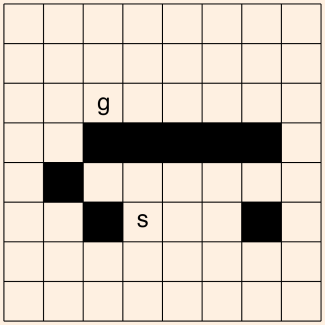
\includegraphics[width=0.35\textwidth]{grid.png}
            \end{figure}
        
            \item No labirinto abaixo, numere os nós expandidos (visitados) por um agente que implementa um algoritmo de busca de Menor custo primeiro.
            \begin{figure}[!ht]
                \centering
                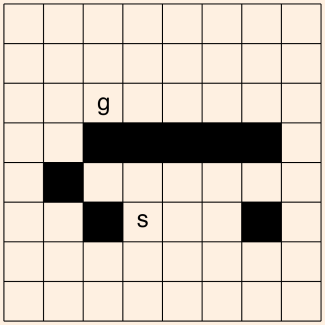
\includegraphics[width=0.35\textwidth]{grid.png}
            \end{figure}
        
            \item No labirinto abaixo, escreva em cada nó o valor da heurística do nó, considerando a distância de Manhattan. Considere que cada quadrado tem lado 1 u.m.
            \begin{figure}[!ht]
                \centering
                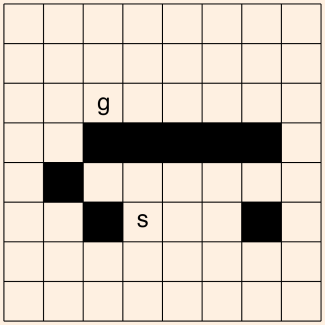
\includegraphics[width=0.35\textwidth]{grid.png}
            \end{figure}
            
            \item No labirinto abaixo, numere os nós expandidos (visitados) por um agente que implementa um algoritmo guloso pela heurística calculada acima. Assuma poda de ciclos.
            \begin{figure}[!ht]
                \centering
                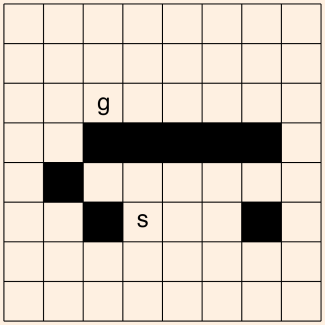
\includegraphics[width=0.35\textwidth]{grid.png}
            \end{figure}
            
            \vspace{2cm}
            
            \item (1pt) No labirinto abaixo, numere os nós expandidos (visitados) por um agente que implementa o algoritmo $A^*$ considerando a distância de Manhattan como custo e heurística.
            \begin{figure}[!ht]
                \centering
                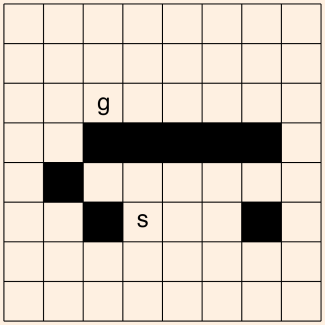
\includegraphics[width=0.35\textwidth]{grid.png}
            \end{figure}
            
        \end{enumerate}

\end{enumerate}

\section{Trabalho Prático}

Neste trabalho, você irá modificar os arquivos \texttt{agents.py} e \texttt{environment.py} para resolver o problema de encontrar um caminho em um labirinto bidimensional, representado como uma matriz.

\subsection*{Descrição do Problema}

O labirinto será representado por uma matriz $m \times n$, onde cada célula pode conter:

\begin{itemize}
    \item \texttt{0}: espaço livre;
    \item \texttt{1}: parede (bloqueio);
    \item \texttt{s}: posição inicial;
    \item \texttt{g}: posição objetivo.
\end{itemize}

O agente pode se mover para cima, baixo, esquerda ou direita, desde que o movimento não ultrapasse os limites da matriz nem atravesse uma parede.

\subsection*{O que deve ser feito}

\begin{enumerate}
    \item Modifique o arquivo \texttt{environment.py}, adicionando uma nova classe chamada \texttt{MazeEnvironment}, que:
    \begin{itemize}
        \item Receba uma matriz como entrada;
        \item Identifique automaticamente a posição inicial (\texttt{s}) e a posição objetivo (\texttt{g});
        \item Implemente o método \texttt{get\_neighbors(state)} que retorna apenas os vizinhos válidos de uma célula.
    \end{itemize}

    \item Modifique as classes \texttt{BFS} e \texttt{DFS} do arquivo \texttt{agents.py} para funcionarem com posições no formato \texttt{(linha, coluna)}.

    \item Teste sua implementação utilizando o arquivo \texttt{maze\_simulation.py}, que será fornecido. Este arquivo:
    \begin{itemize}
        \item Cria um labirinto de exemplo;
        \item Executa o algoritmo de busca (BFS ou DFS);
        \item Imprime o caminho encontrado;
        \item Mostra o labirinto original com o caminho marcado com o símbolo \texttt{*}.
    \end{itemize}
\end{enumerate}

\subsection*{Dicas}

\begin{itemize}
    \item Use uma representação de posições como tuplas: \texttt{(linha, coluna)};
    \item Faça uma cópia da matriz original para marcar o caminho encontrado;
    \item A função \texttt{get\_neighbors} deve verificar se a nova posição está dentro da matriz e se não é uma parede;
\end{itemize}

\subsection*{Entrega}

No seu repositório do GitHub você deve criar um pasta "TrabalhoPraticoBusca" que deve conter:
\begin{itemize}
    \item \texttt{agents.py} modificado;
    \item \texttt{environment.py} modificado;
    \item O arquivo \texttt{maze\_simulation.py} fornecido para testes.
\end{itemize}

O professor dará instruções de como enviar o link do repositório durante a aula. 

\end{document}

